\section{Placement and Routing} \label{sec:par}
The input to the \emph{placement and routing (PaR)} phase is a VUDFG, with each VU tagged to a type of PU.
Before PaR, \name also performs a runtime analysis of the program, annotating each edge in VUDFG
with a link priority. The link priority is used to determine the routing order during PaR.
PaR then iteratively places VUs and route edges in VUDFG onto the global network.

In addition to the original static network in Plasticine, we introduce a dynamic network in
parallel to the static network, forming a dynamic-static hybrid network.
Both purely static and purely dynamic networks are instances of the parameterized hybrid network.
\Cref{sec:network} will discuss the details about the hybrid network.
The PaR algorithm needs to handle both network types and multiple network granularity (vector,
scalar, control) at the same time.

The major difference between the static and the dynamic network is that each physical link in the static network is dedicated to a logical edge in the VUDFG for the entire duration of the execution
(circuit-switching\footnote{Technically, our static network is more restrictive than
circuit-switching because circuit-switching allows deallocation after the connection is terminated.
Our static network, on the other hand, cannot be reconfigured until the application terminates.}), whereas 
the physical link in the dynamic network can be time-shared by multiple logical edges
(packet-switching).
Both static and dynamic networks are statically routed by the PaR algorithm. 
For a dynamic network, PaR also needs to assign virtual channels (VCs) to prevent network deadlock.
The PaR algorithm configures the lookup table in each router that maps the packet header to the
destination port and VC.

In the rest of this section, \Cref{sec:place} and \Cref{sec:route} discusses the placement 
and the routing algorithm. 
\Cref{sec:vc} explains the need for VC allocation. 
Lastly, \Cref{sec:heuristic} describes how \name generates link priority.

\subsection{Iterative Placement} \label{sec:place}

At high-level, the PaR algorithm works very similarly to the FPGA PaR algorithm using
simulated annealing~\cite{simanneal}. 
For the initial placement, the algorithm places VUs in VUDFG in topological order.
Each VU is placed to the next available PU with minimum Manhattan distance to the placed
neighbors of that VU.
Next, the algorithm routes all edges in the VUDFG, starting from edges with the highest link
priority. If no routes are available on the static network, the route will be moved onto the dynamic
network. For purely static networks, there is an ``imaginary'' dynamic network for this step.
At the end of the PaR, if there are still routes on the fake dynamic network, PaR is considered
failed for the static network.
After all routes are routed, either on the static or dynamic network, the PaR evaluates the
congestion cost of the current placement.
Then, a genetic algorithm shuffles the VUs whose edges contribute most to congestion, 
and keeps the new position if it improves the route assignment.
By iteratively re-placing and re-routing, the mapping process eventually converges to a good placement.

The PaR uses a heuristic cost model to rapidly evaluate placements: a 
penalty score is assigned as a linear function of several subscores.
These include projected congestion on dynamic links, projected congestion at network injection and ejection ports, the average route length, and the length of the longest route.
\name provides a static estimate of the number of packets sent on each logical link.
The PaR algorithm estimates congestion by normalizing the number of packets on each link to the program link with the highest total packet count.
The most active program link sets a lower bound on the program runtime (the highest bandwidth physical link can still only send one packet per cycle), which translates to an upper bound on congestion for other links.

%The {\sc Unplace} function randomly decides between unplacing a random node, and unplacing one or several nodes based on heuristics.
%For the heuristic-based unplacement, a node's contribution to global route congestion is calculated by adding an estimate of all connected routes' contributions to the global penalty score; the node(s) with the highest scores are unplaced.
%Similarly, {\sc Place} also can either randomly place an unplaced node, or place it to minimize the Manhattan distance to its logical neighbors. {\sc Score} calculates the heuristics for each node, and {\sc Filter} duplicates the best candidate placements to fill the pool. Because the unplacement and replacement steps can make a placement worse, the best performing placements are frozen in each iteration to ensure that no good placements are thrown away.

\subsection{Congestion-Aware Routing} \label{sec:route}
%\info{Somewhere we should mention that placement and routing running interchangeably}
To achieve optimal performance, we use a routing algorithm that projects congestion and routes around it. 
Routing starts with the highest-priority routes, as determined by fanout of the broadcast edge and
estimated packet count; broadcast edge with higher fanout is harder to route and hence are routed
first.
Using the packet count as a priority makes sure that the static network is used most efficiently.
Our scheme searches a large space of routes for each link, using Dijkstra's algorithm \cite{dijkstra} and a hop weighting function.
To ensure maximum link reuse in broadcast edges, we can augment the hop weight in Dijkstra's
algorithm by a multiplication factor between zero and one. 
When finding the shortest path between each source-destination pair, the weight of the hop is
multiplied by the factor each time the hop is reused for the same broadcast edge.
In other words, the reused path has a lower hop cost compared to other paths.
This trick provides a balance between the shortest path and link reuse: a smaller factor encourages link
reuse, even though individual source-destination pairs are not the shortest path; a factor equals to 1 ensure all source-destination pairs are routed with the shortest path.
The other objective for routing broadcast links is balancing the hop counts between all
destinations. This is because the shorter path will back pressure the sender before packets reaching to the longer path, causing pipeline stalls.
To achieve this, we start with the source-destination pair with the longest Manhattan distance, ensuring
the most far apart source-destination pair is routed on the shortest path.
The consecutive source-destination pairs will try sharing the link on this path and slightly detour from
their shortest path, which balances the hop count.
%Routes are not analyzed on the basis of a single source-destination pair, which would be inadequate for broadcasts: instead, a directed graph is built from the source and all destinations in the route, with edge weights corresponding to the minimal route between each pair of VUs in the broadcast.
%For example, if the broadcast is from VU-1 to VU-2 and VU-3, four total potential routes are analyzed for congestion: VU-1 to VU-2, VU-1 to VU-3, VU-2 to VU-3, and VU-3 to VU-2.
%The routes are weighted so that routes mapped on the static network are preferable to those mapped to the dynamic network; within these categories, routes are weighted based on length. 

%\info{does the nodes refer to only source and destinations or including all nodes on the path between source and destination. How does the weights represent the minimum routes? Is it capturing the cost of the minimum route?}
%Then, a search algorithm based on Prim's algorithm for minimum spanning trees \cite{prim1957shortest} is run to build a tree for the broadcast, starting with only the source being reached.
%At every step, the most-preferable route (from the graph built using Dijkstra's algorithm) that adds a new destination VU to the reached set is chosen and added to the broadcast, until all destination VUs are reached. 
%This route can start from either the source of the broadcast tree or any destination currently in the reached set.
%The algorithm will find a fully static broadcast tree, if one exists, and will only add a non-static route to the broadcast (moving the entire broadcast to the dynamic network) when there are VUs in the tree that cannot be reached from the source VU by \emph{any} static route.
%\info{does the algorithm routes links from high priority to low from all nodes or it does one node at a time?}

\subsection{VC Allocation for Deadlock Avoidance} \label{sec:vc}
Deadlock is a system pathology in dynamic routing where multiple flits form a cyclic holds on/waits for dependency on each others' buffers and prevent forward progress.
Most dataflow accelerators use a streaming model, where outputs of a producer are sent over the network to one or more consumers
without an explicit request; the producer is backpressure when there is insufficient buffer space. 
While this paradigm improves accelerator throughout by avoiding the round-trip delay of a request-response protocol, it introduces an additional source of deadlock \cite{hansson2007avoiding}. 

\Cref{fig:deadlock}(a) shows a sample VUDFG graph, which is statically placed and routed on a $2\times3$ network in (b). 
Logical edges B and C share a physical link in the network. If C fills the buffer shared with B, VU-3 will never receive any packets from B and will not make forward progress.
%For y-z dimension-order routing, the only valid routes from VU-1 to VU-3 is through $\[0,1\], \[0,0\], \[1,0\], \[2,0\]$. 
%Dimension-order routing prevents deadlock by eliminating cycles in network routes.
%On traditional NoCs, deadlock can be solved with dimension-order routing, which routes all traffic on one dimension before another.
%\yaqi{
  With streaming computation, the program graph must be considered as part of the network dependency graph, which must be cycle-free to guarantee deadlock freedom. However, this is infeasible because cycles can exist in a valid VU dataflow graph when the original program has a loop-carried dependency. Therefore, deadlock avoidance using cycle-free routing, such as dimension-order routing, does not work in our scenario. 
Allocating VCs to prevent multiple logical links from sharing the same physical buffer is consequently the most practical option for deadlock avoidance on streaming accelerators.
%Because the entire program is connected through these streaming dependencies, any two links can conflict and result in a deadlock.
%\yaqi{However, cycles are permitted in the programming paradigms since loop-carried dependencies can be mapped across the network.
%Therefore, we perform VC allocation at each router to prevent multiple logical links from sharing the same physical buffer.
\if 0
Virtual channel (VC) allocation is another common approach to avoid deadlock. We can statically assign conflicting streams B and C with different
virtual channels at router $[2,0]$, which prevents them to share physical buffers. 
Notice indirect inputs of a VU, such as A and D with eventual consumer VU-3,
also need distinct VCs to ensure deadlock-free. To minimize the number of VCs required, we perform per-hop VC allocation--statically
assign conflicting links at each input of each router with distinct VCs. The VCs can be looked up at runtime based on link ID.
Distinct links from the same source VU, such as A and C, can share the same VC because VU-1 ensures the number of flits sent over A and C remains
to a ratio that the receiver expects, which permits data to drain in the network.
\fi

\begin{figure}
\centering
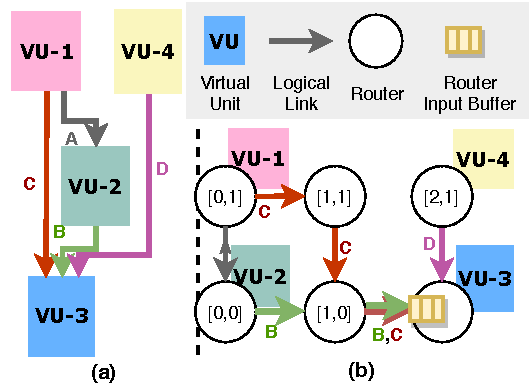
\includegraphics[width=0.4\columnwidth]{figs/deadlock.pdf}
  \caption{An example of deadlock in a streaming accelerator, showing the (a) VU data-flow graph and (b) physical placement and routes on a $2\times3$ network. There are input buffers at all router inputs, but only the buffer of interest is shown.}\small\textsuperscript{}\label{fig:deadlock}
\end{figure}

\subsection{Runtime Analysis for Heuristic Generation} \label{sec:heuristic}

In Spatial, users can annotate the value of runtime variables to assist compiler analysis.  
We use these programmer annotations to compute the expected number of iterations each basic block
will execute. 
The execution count on the basic block can further be used to derive the packet counts produced
by these basic blocks.
For a loop with data-dependent bounds, the user can annotate an estimate of the bound value.
For a branch statement, the user can annotate a percentage distribute between the if and else clauses.
The runtime of a streaming program is a function of the number of packets received on the incoming
stream. 
Static runtime analysis can identify potential application-level deadlock due to stream mismatching, as shown
in \Cref{fig:runtime}.

The derived packet counts based on these annotations can help the placer to evenly spread out the traffic.
The placer prioritizes highly used links on the static network and leaves infrequently used links on the dynamic network. 
However, we do not require exact annotations for efficient placement---rough estimates of these runtime values are sufficient to determine the relative importance of links.
When no annotation is provided, the compiler estimates
loop iteration counts based on the nesting depth: packets generated by the innermost loops are 
the more likely to be frequent.
This heuristic provides a reasonable estimate of links' priorities for routing purposes.

\begin{figure*}
\centering
\begin{subfigure}[b]{0.8\textwidth}
\inputminted{python}{code/runtime.py}
\caption{Example program}
\end{subfigure}
\caption[Runtime Analysis]{
  Example of a streaming program whose runtime depends on the number of packets received on
  \texttt{stream}. We use a \texttt{queue} to model a stream receiving the packets from the
  network.
  Loop \emph{A} is a forever loop whose runtime is determined by its child controllers.
  With user annotation on number of packets from \texttt{stream}, 
  we know the runtime of loop \emph{B} is $T(B) = N$.
  As a result, we can derive the runtime of loop \emph{B}'s and parent \emph{A}, 
  i.e. $T(A) = \lceil\frac{N}{B}\rceil$. 
  With runtime for $A$, the runtime for $C$,$D$,and $E$ can be computed as
  $T(C) = \lceil\frac{N}{B}\rceil\cdot C$,
  $T(D) = \lceil\frac{N}{B}\rceil\cdot C \cdot R$, 
  and $T(E) = \lceil\frac{N}{B}\rceil\cdot C \cdot R \cdot E$.
  The runtime for \emph{E} also depends on \texttt{q}, which gives $T(E) = T(B) = N$. 
  If $\lceil\frac{N}{B}\rceil\cdot C \cdot R \cdot E \neq N$, \name gives an warnning for the
  inconsistency that potentially triggers an undesired deadlock.
}
\label{fig:msr}
\end{figure*}
